\chapter{Optical tracking system}\label{tracking_system}

\begin{figure}[tbh]
    \centering
    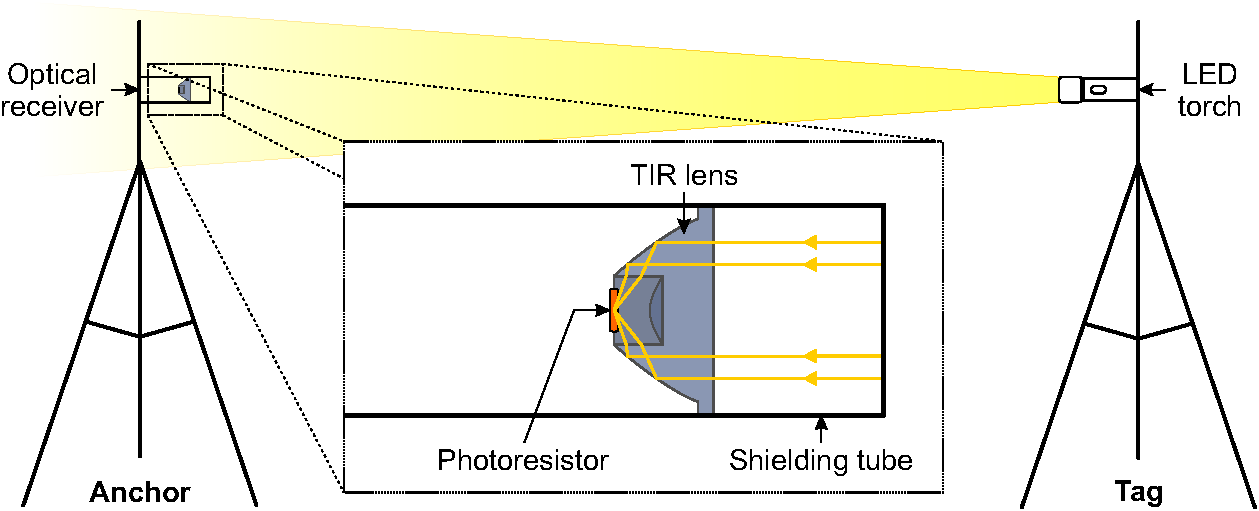
\includegraphics[width=0.9\textwidth]{Figures/appendices/tracking_system.pdf}
    \caption{Schematics of the proposed optical LoS tracking system.}
    \label{fig:tracking_system}
\end{figure}

A custom optical detection system, shown in \autoref{fig:tracking_system}, was implemented at each anchor to enable automated LoS labeling during data collection. The system works by detecting the presence of a direct optical link between the tag and anchors.

Each anchor was equipped with a photoresistor housed in a light-shielding tube to reduce ambient light interference. To enhance angular selectivity and signal-to-noise ratio, we placed a receiving lens at the tube entrance to concentrate incident light onto the photoresistor. We used a total internal reflection (TIR) collimator lens, commonly found in LED optics, for its narrow acceptance angle, wide availability, and low cost. Specifically, a \SI{30}{\degree} TIR lens was selected to effectively suppress off-axis illumination.

The tag was fitted with narrow-beam LED torches, each aligned with the respective anchor's receiver axis. LoS was inferred when the incoming light was detected at the receiver; NLoS was indicated by a drop in received intensity. For digital classification, the photoresistor at each anchor was integrated into a voltage divider connected to a digital input pin. A pull-down resistor value was empirically tuned to set the detection threshold. The resulting binary signal was sampled in sync with the ranging exchange (see \autoref{theory:twr}) and relayed to the tag, enabling real-time classification.

\section{Practical considerations}
In practice, the angular resolution of the proposed system is limited due to the formation of penumbra region near occlusion boundaries, leading to ambiguity in classification. Although the optical behavior in this region is too complex for precise analytical modeling, our isolated empirical study based on ranging error analysis shows the system achieves a sensitivity of \SI{\approx 96}{\percent} and specificity of \SI{\approx 83}{\percent}, indicating that it reliably detects true NLoS conditions while conservatively labeling some LoS cases as NLoS. This bias toward reliability over precision may be acceptable in scenarios where underestimating channel degradation is more harmful than overestimating it, but the resulting limitation should be carefully considered in downstream applications. While we acknowledge that a laser-based solution could offer improved resolution due to its highly collimated beam, it would also pose safety concerns and increase alignment complexity. We therefore opted for an LED-based design as a balanced alternative.
